%--------------------------------------------------------------
% thesis.tex 
%--------------------------------------------------------------
% Corso di Laurea in Informatica 
% - template for the main file of Informatica@Unifi Thesis 
% - based on Classic Thesis Style Copyright (C) 2008 
%   Andr\'e Miede http://www.miede.de   
%--------------------------------------------------------------
\documentclass[twoside,openright,titlepage,fleqn,
	headinclude,12pt,a4paper,BCOR=5mm,footinclude]{scrbook}

\usepackage[nottoc]{tocbibind}
%--------------------------------------------------------------
% Inputs for the title page 
%--------------------------------------------------------------
\newcommand{\myItalianTitle}{Titolo italiano\xspace}
\newcommand{\myEnglishTitle}{English title\xspace}
% use the right myDegree option
\newcommand{\myDegree}{Corso di Laurea in Informatica\xspace}
%\newcommand{\myDegree}{Corso di Laurea Magistrale in Informatica\xspace}
\newcommand{\myName}{Candidate's Name Surname\xspace}
\newcommand{\mySupervisorTitle}{Relatore/Relatrice\xspace} %%% remove one of the two
\newcommand{\mySupervisorName}{\textit{Supervisor's Name Surname}\xspace} 
\newcommand{\myCoSupervisorTitle}{Correlatore/Correlatrice\xspace} %%% optional: remove this command if the thesis has no Co-Supervisor
\newcommand{\myCoSupervisorName}{\textit{Co-Supervisor's Name Surname}\xspace} %%% optional: remove this command if the thesis has no Co-Supervisor
\newcommand{\myTime}{Anno Accademico 202X-202Y\xspace}
%--------------------------------------------------------------


\usepackage{minted}

\usepackage[utf8]{inputenc} 
\usepackage[T1]{fontenc} 

% switch italian and english, depending on the language of the thesis
% this will change the chapter titles
%\usepackage[italian]{babel}
\usepackage[english]{babel}
\usepackage{csquotes}
\usepackage{comment}
\usepackage[fleqn]{amsmath}  
\usepackage{ellipsis}
\usepackage{listings}
\usepackage{subfig}
\usepackage{caption}
\usepackage{appendix}
\usepackage{siunitx}
\usepackage[pdftex]{graphicx} 
\graphicspath{{./Figures/}}
 \usepackage[eulerchapternumbers,linedheaders,subfig,beramono,eulermath,
parts,dottedtoc]{classicthesis}

\captionsetup[listing]{name=Listato}
\captionsetup[figure]{name=Figura}
%--------------------------------------------------------------
% Layout setting
%--------------------------------------------------------------
\newlength{\abcd} 
\newcommand{\myfloatalign}{\centering} 
\setlength{\extrarowheight}{3pt} 
\captionsetup{format=hang,font=small}

\usepackage{geometry}
\geometry{
	a4paper,
	ignoremp,
	bindingoffset = 1cm, 
	textwidth     = 13.5cm,
	textheight    = 21.5cm,
	lmargin       = 3.5cm, 
	tmargin       = 4cm    
}

\lstset{
  	frame=tb,
	language=Matlab,
  	aboveskip=3mm,
  	belowskip=3mm,
  	showstringspaces=false,
  	columns=flexible,
  	basicstyle={\small\ttfamily},
  	numbers=none,
  	breaklines=true,
  	breakatwhitespace=true,
  	tabsize=3
}

%--------------------------------------------------------------
\begin{document}
\frenchspacing
\raggedbottom
\pagenumbering{roman}
\pagestyle{plain}
%--------------------------------------------------------------
% Frontmatter
%--------------------------------------------------------------
\include{FrontMatter/Titlepage}
\pagestyle{scrheadings}
%--------------------------------------------------------------
% Mainmatter
%--------------------------------------------------------------
\pagenumbering{arabic}
\tableofcontents
\listoffigures
\cleardoublepage
\thispagestyle{empty}
\begin{flushright}
\null\vspace{\stretch {1}}
%--------------------------------------------------------------
% Citation
%--------------------------------------------------------------
\emph{"Se avessi avuto più tempo, avrei scritto una lettera più breve." \break --- Blaise Pascal} \vspace{\stretch{2}}\null
\end{flushright}
\cleardoublepage

%--------------------------------------------------------------
% Chapters
%--------------------------------------------------------------
% !TEX root = ../Thesis.tex

\chapter{Introduction}

The introduction is usually a short chapter that can be read in less than 10 minutes.

The goal of the Introduction is to engage the reader (why you should keep reading).
You don't have to discuss anything in detail. Rather, the goal is to tell the reader:
\begin{itemize}
%  \item Why something has to be done (why the thesis topic is important),
  \item what is the problem dealt with and why the problem is a problem;
  \item what is the particular topic you're going to talk about in the thesis;
  \item what are your goals in doing so, and what methodology do you follow;
  \item what are the implications of your work.
\end{itemize}

The above points will be further expanded in the following chapters, so only a glimpse is essential. 

\medskip

It is customary to conclude the Introduction with a summary of the content of the rest of the thesis. One or two sentences are enough for each chapter.
% !TEX root = ../Thesis.tex

\chapter{Gestione della memoria}

\section{L'approccio di Java}
Java è un linguaggio di programmazione progettato per essere semplice da usare e portabile, con una gestione della memoria che mira a garantire sicurezza e facilità d'uso a scapito di un controllo diretto da parte del programmatore. Java raggiunge questi obiettivi principalmente attraverso l'uso di un \textit{garbage collector} e un ambiente di esecuzione controllato (la Java Virtual Machine - JVM). Gli aspetti fondamentali dell'approccio di Java sono:

\begin{enumerate}
\item La gestione automatica della memoria tramite il garbage collector, che si occupa di identificare e liberare la memoria occupata da oggetti non più raggiungibili nel programma, prevenendo così problemi comuni, come i memory leak. Questo, di fatto, toglie al programmatore la responsabilità collegata al dover gestire manualmente l'allocazione e la deallocazione della memoria, riducendo la probabilità di errori nel codice.
\item La prevenzione di comportamenti indefiniti principalmente a run-time, attraverso un controllo rigoroso dell'accesso alla memoria e la gestione delle eccezioni. 
\end{enumerate}

Sebbene l'approccio di Java renda lo sviluppo più semplice e sicuro rispetto a linguaggi senza garbage collector, come C e C++, l'uso del garbage collector introduce una certa imprevedibilità nelle prestazioni, in quanto il processo di garbage collection deve essere eseguito in concorrenza con l'esecuzione del programma. 
\section{L'approccio di Rust}
Rust è un linguaggio di programmazione che si distingue per la sua gestione della memoria, evitando la necessità di un garbage collector e garantendo al contempo sicurezza e prestazioni elevate. Rust ha due obiettivi principali:
\begin{enumerate}
    \item  Garantire che il programma sia privo di comportamenti indefiniti, ovvero situazioni in cui il programma può agire in modo imprevedibile. Un esempio tipico è l'accesso a memoria non valida, che può portare all'esecuzione di codice con dati non inizializzati o causare errori di memoria come segmentation fault. 
    \item Prevenire comportamenti indefiniti a compile-time, piuttosto che a run-time. Questo significa che il compilatore di Rust è in grado di rilevare e segnalare errori di memoria prima che il programma venga eseguito, riducendo il rischio di bug e di errori durante l'esecuzione. Inoltre, viene ridotto il numero di controlli a run-time, migliorando le prestazioni del programma. 
    % Nell'articolo di google viene riportato il vantaggio di non avere controlli a run-time.
\end{enumerate}
Rust non può prevenire tutti i bug ma le metodologie messe in atto per la gestione della memoria rendono un programma scritto in Rust molto più sicuro rispetto a uno scritto in linguaggi con meno controlli. 

Un esempio concreto dell'efficacia di Rust nella prevenzione degli errori di memoria è fornito da Google \cite{android13-memorysafe}, che ha introdotto il linguaggio nello sviluppo di Android 13. In particolare, circa il 21\% del nuovo codice introdotto in Android 13 è stato scritto in Rust, e, alla data della pubblicazione dell'articolo, sono state scoperte zero vulnerabilità di sicurezza legate alla memoria in questo codice. Questo è un risultato significativo che dimostra come gli obiettivi prefissati da Rust siano stati raggiunti nella pratica.

Rust realizza questi obiettivi attraverso un sistema basato sui concetti di \textit{ownership} e \textit{borrowing}. Concetti fondamentali che verrano affrontati in dettaglio nelle prossime sezioni.

\section{Stack e Heap}
Sia Java che Rust utilizzano due aree di memoria principali: lo stack e l'heap, ma la loro gestione è profondamente diversa, riflettendo i diversi modelli di memoria adottati dai due linguaggi.

Lo stack è un'area di memoria strutturata con una struttura dati stack LIFO (Last In, First Out). La memoria stack è contigua e i dati memorizzati al suo interno sono in posizione fissa rispetto allo stack pointer, un puntatore che punta all'ultimo elemento inserito. Questo permette un accesso rapido ai dati usando indirizzi di memoria calcolati in modo semplice tramite un offset rispetto allo stack pointer. Inoltre, allocazione e deallocazione della memoria stack sono molto veloci poiché avvengono spostando lo stack pointer, avanti o indietro, di un numero di byte opportuno rispetto alla dimensione del dato e all'architettura della CPU.

L'heap, al contrario, è un'area di memoria non strutturata, in cui i dati possono essere allocati in qualsiasi sua posizione. L'allocazione e la deallocazione della memoria heap richiedono operazioni più complesse rispetto allo stack, poiché il sistema operativo deve tenere traccia degli spazi liberi e occupati. Questo può portare a un utilizzo meno efficiente della memoria (frammentazione) e a un accesso più lento ai dati rispetto allo stack. 

In Java, l'allocazione della memoria è fortemente automatizzata. Ogni volta viene creato un oggetto, tramite la keyword \texttt{new}, viene allocata memoria heap nel quale sarà memorizzato l'oggetto. L'uso dello stack è limitato a variabili di tipo primitivo e variabili locali. Al contrario, Rust adotta un modello più esplicito e flessibile. In rust, la variabili possono essere allocate sia nello stack che nell'heap, a seconda dalla conoscenza a compile time delle dimensioni del dato:
\begin{itemize}
    \item  Se la variabile ha una dimensione fissa nota a compile time, viene allocata nello stack. É possibile allocare nell'heap anche variabili di dimensione fissa attraverso \texttt{Box}.
    \item  Se la variabile ha una dimensione variabile o non nota a compile time, viene allocata nell'heap. 
\end{itemize} 
Questa è una differenza fondamentale rispetto a Java, perchè permette allo sviluppatore di avere più controllo su dove vengono allocati i dati, permettendo ottimizzazioni specifiche per le esigenze del programma. 

Ad esempio, sia in Java che in Rust, gli array hanno una dimensione fissa. Tuttavia, in Java, gli array sono allocati nell'heap e sono referenziati da variabili nello stack, mentre in Rust, poiché si conosce la loro dimensione a compile time, vengono allocati nello stack. Questo rende l'accesso agli elementi dell'array di Rust più veloce. 
\begin{minted} [fontsize=\small] {Java}
    int[] arr = {1, 2, 3, 4, 5}; // Array allocato nell'heap
    System.out.println("Il primo elemento e': " + arr[0]);
\end{minted}
\begin{minted} [fontsize=\small] {Rust}
    let arr = [1, 2, 3, 4, 5]; // Array allocato nello stack
    println!("Il primo elemento e': {}", arr[0]);
\end{minted}
\section{Ownership}
L'ownership è un concetto fondamentale in Rust il quale può essere definito come un insieme di regole che il compilatore controlla per garantire una corretta gestione della memoria. Questo significa sia garantire che non ci siano errori di memoria a run-time, sia che la memoria inutilizzata venga rilasciata correttamente per non terminare lo spazio di memoria disponibile (\textit{memory leak}). 

L'obiettivo principale dell'ownership è, quindi, quello di gestire la memoria heap tenendo traccia di quali parti di codice utilizzano valori contenuti in essa, minimizzare valori duplicati e garantire che la memoria venga rilasciata quando non è più necessaria. 
%TODO: Forse inserire confronto con Java su performance e garbage collector 

L'ownership si basa su tre regole principali: 
\begin{enumerate}
    \item  Ogni valore in Rust ha un \textit{owner}, ovvero una variabile che ne detiene la proprietà. 
    \item  Un valore può avere un solo owner alla volta. 
    \item  Quando l'owner di un valore esce dallo scope, il valore viene automaticamente rilasciato dalla memoria.
\end{enumerate}
Consideriamo un caso banale in cui si crea una variabile all'interno di uno scope:
\begin{minted} [fontsize=\small] {Rust}
    {
        let s = String::from("Hello");
    }
\end{minted}
In questo caso, secondo la regola 3, quando la variabile \texttt{s} esce dallo scope, il valore \texttt{"Hello"} viene automaticamente rilasciato dalla memoria. Questo avviene attraverso la funzione \texttt{drop} che viene chiamata automaticamente da rust quando la variabile va fuori dallo scope. In java questo non accade. Dato il seguente codice equivalente in Java:
\begin{minted} [fontsize=\small] {Java}
    {
        String s = "Hello";
    }
\end{minted}
La memoria occupata dalla stringa \texttt{"Hello"} non viene rilasciata automaticamente quando la variabile \texttt{s} esce dallo scope ma solo quando il garbage collector esegue la raccolta dei valori non più raggiungibili. Già da questo semplice caso si può notare come l'ownership di Rust permetta di avere un controllo più preciso sulla memoria. 

Un altro aspetto importante dell'ownership è che, quando si assegna un valore a un'altra variabile, l'ownership viene trasferita. Ad esempio, consideriamo il seguente codice:
\begin{minted} [fontsize=\small] {Rust}
    let s1 = String::from("Hello");
    let s2 = s1; // Ownership di s1 viene trasferita a s2
    // println!("{}", s1); // Errore di compilazione
    println!("{}", s2);
\end{minted}
In questo caso, l'ownership della stringa \texttt{"Hello"} viene trasferita da \texttt{s1} a \texttt{s2}. Dopo il trasferimento, \texttt{s1} non è più valida e qualsiasi tentativo di accedervi causerà un errore di compilazione. 
\begin{figure}[H]
    \label{fig:own1}
    \centering
    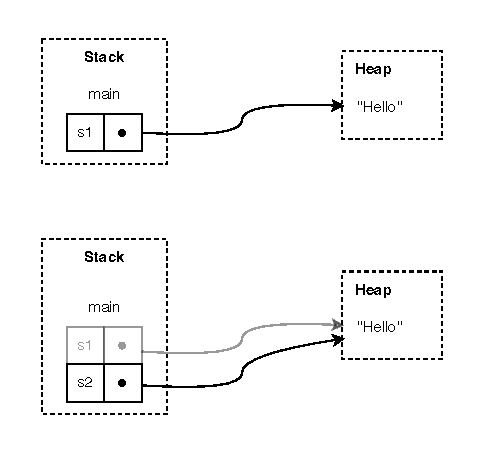
\includegraphics[scale = 1]{Figures/own1.pdf}
    \caption{Visualizzazione memoria Rust dopo il trasferimento di ownership.}
\end{figure}
In Rust, per variabili il cui valore è contenuto in memoria heap, un'istruzione di copia esegue una \textit{shallow copy} del valore e invalida la variabile originale. Questo comportamento prende il nome di \textit{move}. Rust non esegue mai una \textit{deep copy} di una variabile: se il programmatore desidera duplicare effettivamente il contenuto, deve farlo in modo esplicito (ad esempio usando il metodo \texttt{clone()}). Quindi, l'operazione di copia base è poco costosa in termini di performance.

Questo non è consistente con quello che accade in Java, dove l'assegnazione di un oggetto a un'altra variabile non invalida quella originale, ma crea una nuova referenza all'oggetto esistente. Entrambe le variabili possono accedere all'oggetto, condividendono lo stato. In Java, il codice equivalente sarebbe:
\begin{minted} [fontsize=\small] {Java}
    String s1 = "Hello";
    String s2 = s1; 
    System.out.println(s1); // Valido
    System.out.println(s2); // Valido
\end{minted}
In questo caso, quindi, entrambe le stringhe verrebbero correttamente stampate. L'approccio adottato da Rust è decisamente più restrittivo, ma si tratta di una caratteristica desiderabile: consente infatti di evitare errori comuni legati alla gestione della memoria, come l'accesso a variabili non più valide o la modifica involontaria di dati condivisi. 
Ad esempio, in Java, il codice seguente potrebbe causare un comportamento indesiderato:
\begin{minted} [fontsize=\small] {Java}
    class Person {
        String name;
        Person(String name) {
            this.name = name;
        }
    }

    public class Main {
        public static void main(String[] args) {
            Person p1 = new Person("Alice");
            Person p2 = p1; // p2 è una referenza a p1
            p2.name = "Bob"; // Modifica il nome di p1
            System.out.println(p1.name); // Stampa "Bob"
        }
    }
\end{minted}
In questo esempio, la modifica del campo \texttt{name} di \texttt{p2} influisce anche \texttt{p1}, poiché entrambi i riferimenti puntano allo stesso oggetto in memoria. Questo comportamento puà causare bug sottili e difficili da individuare, spcialmente in contesti complessi o concorrenti. In Rust, invece, il trasferimento di ownership impedisce il comportamento appena descritto, poiché una volta che l'ownership è stata trasferita, la variabile originale non può più essere utilizzata.
%TODO: dall'esempio precedente posso passare a rust con passaggio di parametro a funzione

% !TEX root = ../Thesis.tex

\chapter{How to heat the water differently}
\label{cap:proposal}

This is the `main' chapter of your thesis.

Here you have to show that \emph{your} version of heated water differs slightly from any other known version of heated water, and this is important.

\section{How did I discover a novel type of heated water}

Explain in detail what are the steps to heat the water in a novel way.

\section{How my heated water differs from the previous ones}

Describe why and how your findings are different from the past versions.

Here you might want to add code (see for example Listing~\ref{code:example}), or tables (see Table~\ref{tab:example}).

Note that figures, listings, tables, and so on, should never be placed `manually'. Let LaTeX decide where to put them - you'll avoid headaches (and bad layouts). Furthermore, each of them must be referred to at least once in the body of the thesis.


\begin{lstlisting}[language=Python, caption=Python example, float, label=code:example]
import numpy as np
    
def incmatrix(genl1,genl2):
    m = len(genl1)
    n = len(genl2)
    M = None #to become the incidence matrix
    VT = np.zeros((n*m,1), int)  #dummy variable
    
    #compute the bitwise xor matrix
    M1 = bitxormatrix(genl1)
    M2 = np.triu(bitxormatrix(genl2),1) 

    for i in range(m-1):
        for j in range(i+1, m):
            [r,c] = np.where(M2 == M1[i,j])
            for k in range(len(r)):
                VT[(i)*n + r[k]] = 1;
                VT[(i)*n + c[k]] = 1;
                VT[(j)*n + r[k]] = 1;
                VT[(j)*n + c[k]] = 1;
                
                if M is None:
                    M = np.copy(VT)
                else:
                    M = np.concatenate((M, VT), 1)
                
                VT = np.zeros((n*m,1), int)
    
    return M
\end{lstlisting}

\begin{table}[tbp]
\centering
\caption{Example table}
\label{tab:example}
\begin{tabular}{@{}lll@{}}
\toprule
Country       & Country code & ISO codes \\ \midrule
Canada        & 1            & CA / CAN  \\
Italy         & 39           & IT / ITA  \\
Spain         & 34           & ES / ESP  \\
United States & 1            & US / USA  \\ \bottomrule
\end{tabular}
\end{table}


% !TEX root = ../Thesis.tex

\chapter{Numerical results}

This is where you show that the novel `thing' you described in Chapter~\ref{cap:proposal} is, indeed, much better than the existing versions of the same.

You will probably use figures (try to use a high-resolution version), graphs, tables, and so on. An example is shown in Figure~\ref{fig:dave}.

\begin{figure}[htbp]
\begin{center}
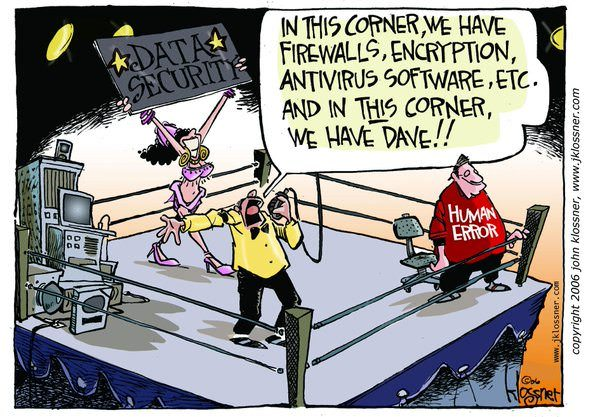
\includegraphics[width=.7\textwidth]{DaveSecurity}
\caption{Network Security - the sad truth}
\label{fig:dave}
\end{center}
\end{figure}

Note that, likewise tables and listings, you shall not worry about where the figures are placed. Moreover, you should not add the file extension (LaTeX will pick the `best' one for you) or the figure path.

% !TEX root = ../Thesis.tex

\chapter{Conclusions and Future work}

They say that the conclusions are the shortened version of the introduction, and while the Introduction uses future verbs (we will), the conclusions use the past verbs (we did). It is basically true.

In the conclusions, you might also mention the shortcomings of the present work and outline what are the likely, necessary, extension of it.
E.g., we did analyse the performance of this network assuming that all the users are pedestrians, but it would be interesting to include in the study also the ones using bicycles or skateboards.

Finally, you are strongly encouraged to carefully spell check your text, also using automatic tools (like, e.g., Grammarly\footnote{\url{https://www.grammarly.com/}} for English language).

%--------------------------------------------------------------
% Bibliography
%--------------------------------------------------------------
%\bibliographystyle{unsrt} Entries are sorted by order of citation
\bibliographystyle{plain} 
\bibliography{Bibliography} % Entries are in the Bibliography.bib file

%--------------------------------------------------------------
\end{document}
%--------------------------------------------------------------
